\documentclass{beamer}

\usepackage[utf8]{inputenc}
\usepackage[ngerman]{babel}

\mode<presentation> {
  %\setbeameroption{show notes} % Kommentare im fertigen PDF

  \usetheme{Boadilla}
  \usecolortheme{seagull}

  \setbeamertemplate{footline}[page number] % Einfacher Folienzähler als Fußzeile
  \setbeamertemplate{navigation symbols}{} % Keine Navigationslinks
}

\usepackage{graphicx} % Zum Bilder-Einbinden

% Damit die Tilde ~ im Code nicht hochgestellt dargestellt wird, muss man einen anderen Font verwenden, z.B.
%\usepackage[T1]{fontenc}
%\usepackage{beramono}
% Dieser Font ist aber zu breit.
% siehe https://github.com/gpoore/minted/issues/2#issuecomment-18451836
\usepackage[outputdir=output]{minted} % Syntax-Highlighted Code; requires pygments to be installed
\newminted{haskell}{}
\newmintinline{haskell}{}

\usepackage{hyperref}
\usepackage{url}

\usepackage{bbm} % Buchstaben mit Doppelstrich
\usepackage[normalem]{ulem} % Durchstreichen

\renewcommand{\O}{\mathcal{O}} % Landau-O
\newcommand{\N}{\mathbbm{N}} % natürliche Zahlen
\newcommand{\ghci}{\textcolor{lightgray}{Prelude>}} % GHCI-Prompt

\definecolor{greenncs}{rgb}{0.0, 0.62, 0.42}

\defbeamertemplate*{title page}{customized}[1][]
{
  \centering
  \usebeamerfont{title}{\LARGE \inserttitle}\par
  \usebeamerfont{subtitle}\usebeamercolor[fg]{subtitle}\insertsubtitle\par
  \bigskip
  \usebeamercolor[fg]{titlegraphic}\inserttitlegraphic\par
  \bigskip
  \usebeamerfont{author}\insertauthor\\[0.5em]
  \usebeamerfont{institute}\insertinstitute\par
  \usebeamerfont{date}\insertdate\par
}

\title[PFDS]{Rein funktionale Warteschlangen}
\titlegraphic{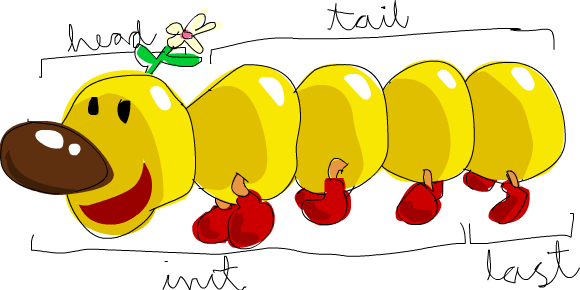
\includegraphics[width=0.65\linewidth]{lyah-caterpillar.png}}
\author{Tim Baumann}
\institute[CCA]{Curry Club Augsburg}
\date{28. Januar 2016}

\begin{document}

\begin{frame}
  \titlepage
\end{frame}

\begin{frame}
  \frametitle{Literatur}
  \begin{itemize}
    \item Standardwerk: Chris Okasaki, \textit{Purely Functional Data Structures}
    \item Artikel von Edsko de Ries auf dem Well-Typed Blog: \\
    \href{http://www.well-typed.com/blog/2016/01/efficient-queues/}{\textit{Efficient Amortised and Real-Time Queues in Haskell}}
  \end{itemize}
  \begin{center}
    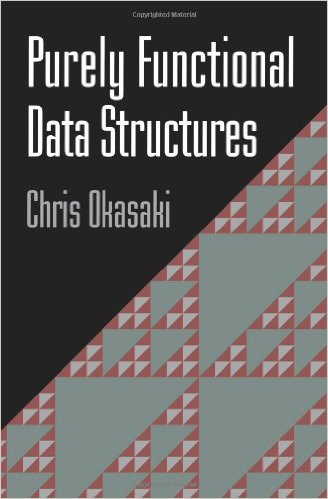
\includegraphics[height=5cm]{pfds_cover.jpg}
  \end{center}
\end{frame}

\begin{frame}[fragile]
  \frametitle{Was sind Warteschlangen?}
  \begin{minipage}[t]{0.57 \linewidth}
\begin{haskellcode}
class Queue q where
  empty  :: q a
  -- hinten anhängen:
  snoc   :: q a -> a -> q a
  -- vorne wegnehmen:
  uncons :: q a -> Maybe (a, q a)
  head :: q a -> Maybe a
  head = fst <$> uncons
  tail :: q a -> Maybe (q a)
  tail = snd <$> uncons
\end{haskellcode}
  \end{minipage}
  \begin{minipage}[t]{0.4 \linewidth}
    \begin{visibleenv}<2->
    Zum Beispiel:
\begin{haskellcode}
instance Queue [] where
  empty = []
  snoc xs x = xs ++ [x]
  uncons []
    = Nothing
  uncons (x:xs)
    = Just (x, xs)
\end{haskellcode}
    \end{visibleenv}
  \end{minipage}
  
  \vspace{0.5cm}

  \begin{itemize}
    \item<3-> \emph{Problem}:
    { \centering \haskellinline{head (snoc (... (snoc empty x1) ...) xn)}} \\
    benötigt $\O(n)$ Zeit in Haskell! In einer strikten Programmiersprache braucht der Aufruf $\text{snoc}(xs, x)$ Zeit $\O(n)$.
    \item<4-> \emph{Ziel}: Eine effiziente Warteschlangen-Datenstruktur für das funktionale Setting entwerfen.
    Die Operationen \haskellinline{snoc} und \haskellinline{uncons} sollen in konstanter Zeit laufen.
  \end{itemize}
\end{frame}

\begin{frame}[fragile]
  \frametitle{Amortisierte Laufzeitanalyse}
  
  Bei der amortisierten Laufzeitanalyse dürfen einzelne Operationen gelegentlich den für sie vorgeschriebenen Zeitrahmen sprengen, solange im Mittel die vorgegebene Zeitschranke eingehalten wird.
  
  \begin{itemize}
    \item<2-> Bankiers-Sichtweise: Es gibt ein (nichtnegatives!) Guthabenkonto. Jede Operation kann Geld abheben ($g < 0$) oder einzahlen ($g > 0$). Die Gesamtkosten einer Operation ist dann $g + t$, wobei $t$ die Laufzeit die Operation ist. Der Kontostand muss zu jedem Zeitpunkt nichtnegativ sein.
    \item<3-> Physiker-Sichtweise: Es gibt eine Potenzialfunktion $\phi : D \to \N$ (wobei $D$ die Menge aller möglichen Zustände einer Datenstruktur ist). Die Kosten einer Operation, die $v \in D$ liest und $w \in D$ produziert, sind $\phi(w) - \phi(v) + t$.
  \end{itemize}
\end{frame}

\begin{frame}[t,fragile]
  \frametitle{Erinnerung: Umdrehen von Listen}
  Man kann eine Liste der Länge~$n$ in Zeit $\O(n)$ umdrehen:
\begin{haskellcode}
reverse :: [a] -> [a]
reverse = go []
  where go as []     = as
        go as (x:bs) = go (x:as) bs
\end{haskellcode}
\end{frame}

\begin{frame}[t,fragile]
  \frametitle{
    Banker's Queues
    \hfill
    \visible<2->{
      \small \color{greenncs}
      \texttt{\{-\# LANGUAGE Strict \#-\}}
    }
  }
  \textit{Idee}: Speichere den vorderen und den hinteren Teil der Liste separat, den hinteren in umgekehrter Reihenfolge (damit man effizient anhängen kann).
  Dabei soll der vordere Teil immer größer als der hintere Teil sein.
  Falls der hintere Teil die gleiche Länge erreicht, so drehe ihn um und hänge ihn an den vorderen Teil an.
\begin{onlyenv}<2>
\begin{haskellcode*}{fontsize=\normalsize}
data BQueue a = BQueue { front :: [a], frontLen :: Int
                       , rear  :: [a], rearLen  :: Int }

empty :: BQueue a
empty = BQueue [] 0 [] 0

mkBQueue :: [a] -> Int -> [a] -> Int
mkBQueue f fl r rl = if
  | fl > rl   = BQueue f fl r rl
  | otherwise = BQueue (f ++ reverse r) (fl + rl) [] 0
\end{haskellcode*}
\end{onlyenv}
\begin{onlyenv}<3>
\begin{haskellcode*}{fontsize=\normalsize}
data BQueue a = BQueue { front :: [a], frontLen :: Int
                       , rear  :: [a], rearLen  :: Int }
-- mkBQueue :: [a] -> Int -> [a] -> Int

uncons :: BQueue a -> Maybe (a, BQueue a)
uncons (BQueue [] _ _ _)       = Nothing
uncons (BQueue (x:xs) fl r rl) =
  Just (x, mkBQueue xs (fl-1) r rl)

snoc :: BQueue a -> a -> BQueue a
snoc (BQueue f fl r rl) x = mkBQueue f fl (x:r) (rl+1)
\end{haskellcode*}
\end{onlyenv}

\begin{onlyenv}<4->
  \vspace{0.5cm}
  \textit{Laufzeitanalyse}: Umdrehen der hinteren Liste und Anhängen an die vordere Liste dauert $\O(n)$ Zeit.
  Falls kein Umdrehen der Liste erforderlich ist, so benötigen \haskellinline{uncons} und \haskellinline{snoc} konstante Zeit.
  \only<4-5>{Bevor das nächste Mal umgedreht werden muss, müssen weitere $n$ Operationen ausgeführt werden.}\only<6->{\sout{Bevor das nächste Mal umgedreht werden muss, müssen weitere $n$ Operationen ausgeführt werden.}}
  Wenn wir für jede dieser Operationen ein oder zwei Geldstücke in das Guthabenkonto legen, können wir für das nächste Mal Umdrehen bezahlen.
\end{onlyenv}

\begin{onlyenv}<5->
  \vspace{0.5cm}
  {\color{red} Dieses Argument ist falsch!}
  \only<6->{Dieser Satz stimmt nicht im funktionalen Setting: Alte Zustände der Datenstruktur werden aufgehoben, es gibt mehrere Zukünfte!}
\end{onlyenv}
\end{frame}

\begin{frame}[t,fragile]
  \frametitle{Lazyness to the rescue!}

  Interpretieren wir den Code der Banker's Queue in gewöhnlichem, nicht-strikten Haskell, so haben \haskellinline{snoc} und \haskellinline{uncons} tatsächlich amortisiert konstante Laufzeit!

  (Grund: \haskellinline{reverse rear} wird nicht sofort berechnet und das Ergebnis wird gespeichert. Beispiel: Amortized Queue)
\end{frame}

\begin{frame}[t,fragile]
  \frametitle{Real-Time Queues}
  Wir wollen nun erreichen, dass \haskellinline{snoc} und \haskellinline{uncons} echt konstante Laufzeit besitzen (nicht nur amortisiert).

  Dazu müssen wir das Umdrehen der hinteren Liste in Teilschritte konstanter Zeit zerlegen.
  Wir verbinden das Umdrehen mit dem Durchlaufen der vorderen Liste:

  \begin{onlyenv}<2->
\begin{haskellcode}
-- `appendAndReverse xs ys zs = xs ++ reverse ys ++ zs`
-- Vorbedingung: `length xs = length ys`
appendAndReverse :: [a] -> [a] -> [a] -> [a]
appendAndReverse []     []     zs = zs
appendAndReverse (x:xs) (y:ys) zs =
  x : appendAndReverse xs ys (y:zs)
\end{haskellcode}
  \end{onlyenv}

  \begin{onlyenv}<3>
\begin{haskellcode}
  appendAndReverse [1,2,3] [6,5,4] [7,8,9]
= 1 : appendAndReverse [2,3] [5,4] [6,7,8,9]
= 1 : 2 : appendAndReverse [3] [4] [5,6,7,8,9]
= 1 : 2 : 3 : appendAndReverse [] [] [4,5,6,7,8,9]
= [1,2,3,4,5,6,7,8,9]
\end{haskellcode}
  \end{onlyenv}

  \begin{onlyenv}<5>
    \textit{Idee}: Führe bei jeder \haskellinline{snoc} und \haskellinline{unsnoc}-Operation einen Teilschritt aus.
    Wir forcieren Teilschritte, indem wir die Ergebnisliste von \haskellinline{appendAndReverse xs ys zs} durchlaufen.
  \end{onlyenv}
\end{frame}

\begin{frame}[t,fragile]
  \frametitle{Real-Time Queues}
\begin{haskellcode}
-- `appendAndReverse xs ys zs = xs ++ reverse ys ++ zs`
appendAndReverse :: [a] -> [a] -> [a] -> [a]
\end{haskellcode}
{\noindent \color{gray} \rule{\textwidth}{0.4pt}}\begin{haskellcode}
data RTQueue a =
  RTQueue { front :: [a], rear :: [a], schedule :: [a] }
-- Invariant: length front = length rear + length schedule
\end{haskellcode}

  (Damit sind die vordere und hintere Liste genau dann gleich lang, wenn \haskellinline{schedule} leer ist.
  Wir müssen also die Längen von \haskellinline{front} und \haskellinline{rear} nicht explizit speichern.)

\begin{haskellcode}
empty :: RTQueue a
empty = RTQueue [] [] []

mkRTQueue :: [a] -> [a] -> [a] -> RTQueue a
mkRTQueue f r [] = let f' = appendAndReverse f r []
                   in RTQueue f' [] f'
mkRTQueue f r (_:s') = RTQueue f r s'
\end{haskellcode}

\end{frame}

\begin{frame}[t,fragile]
  \frametitle{Real-Time Queues}
\begin{haskellcode}
data RTQueue a =
  RTQueue { front :: [a], rear :: [a], schedule :: [a] }
-- Invariante: length front = length rear + length schedule

mkRTQueue :: [a] -> [a] -> [a] -> RTQueue a
mkRTQueue f r [] = let f' = appendAndReverse f r []
                   in RTQueue f' [] f'
mkRTQueue f r (_:s') = RTQueue f r s'
\end{haskellcode}
{ \noindent \color{gray} \rule{\textwidth}{0.4pt}}\begin{haskellcode}
uncons :: RTQueue a -> Maybe (a, RTQueue a)
uncons (RTQueue []     _ _) = Nothing
uncons (RTQueue (x:f') r s) =
  Just (x, mkRTQueue f' r s)

snoc :: RTQueue a -> a -> RTQueue a
snoc (RTQueue f r s) x = mkRTQueue f (x:r) s
\end{haskellcode}
\end{frame}

{\setbeamertemplate{background}{
\includegraphics[width=\paperwidth,height=\paperheight,keepaspectratio]{lyah-caterpillar-end-bg.png}}
\begin{frame}[fragile]
\begin{haskellcode*}{fontsize=\Large,escapeinside=||}
|\ghci| uncons presentation
Nothing :: Maybe (Slide, RTQueue Slide)
\end{haskellcode*}

\vspace{6cm}

{
  \color{gray}
  Interaktive Demo: \href{http://timbaumann.info/pfds-visualizations/}{\textit{timbaumann.info/pfds-visualizations}} \\
  Tausendfüßler-Bild: Miran Lipovača, \textit{Learn You a Haskell for Great Good!}
}
\end{frame}
}

\end{document}
